\chapter{Implementation}
\label{Implementation}

In this chapter, we are going to describe the way we solved the obstacles that we faced during the development stage.

In \chapref*{Technologies} we already named the key frameworks and techniques that we used in the implementation for the client. The server is going to provide to the client a RESTful\footnote{REST or Representational State Transfer is a set of design principles, which make the network communication more flexible and scalable\cite{40}.} interface for the use cases, which we will describe below.

\begin{figure}[!htb]
    \begin{center}
    \setlength{\fboxsep}{4pt}%
    \setlength{\fboxrule}{1pt}%
    \stackunder{\fbox{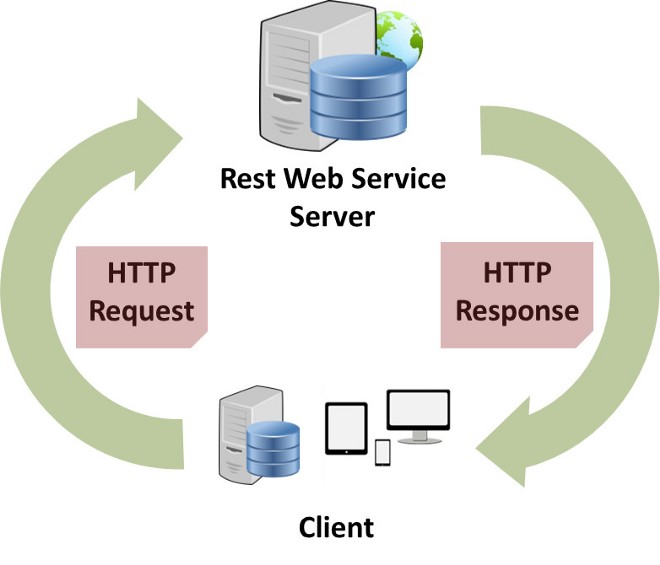
\includegraphics[width=0.5\linewidth]{images/design/clientserver.jpeg}}}%
    {\scriptsize%
     Source: \url{https://cdn-images-1.medium.com/max/660/1*EbBD6IXvf3o-YegUvRB_IA.jpeg}}
    \caption {A server-client architecture with a RESTful interface.}
    \label{fig:design1}
\end{center}
\end{figure}

To demonstrate the functionality of WebCure, we implemented three different types of CRDTs used in AntidoteDB: a counter, a set and a multi-value register. We support each of these data types on the server and the client as well. We will use a Set CRDT as an example for code listings introduced further.

\section{Main components of the system}
\label{sysmaincomponents}

\begin{figure}[!htb]
    \begin{center}
        \setlength{\fboxsep}{15pt}%
        \setlength{\fboxrule}{1pt}%
    \def\svgwidth{\linewidth}
    \fbox{\input{images/design/Main.pdf_tex}}
    \caption {A top-level view of the system's design.}
    \label{fig:impl1}
\end{center}
\end{figure}

In \chapref*{Design}, we introduced a client and a server as black boxes, without really explaining their internal structure. However, we have a clear picture of what the system and its main components will look like. As we can see in \figref*{fig:impl1}, the client part of the system, which we introduced before, contains a web application that has a database on its side for reading and storing the data locally. The server, on the other hand, is controlling an AntidoteDB database and, apart from that, can exchange messages with clients. A service worker controls the communication with the server on a client side. It serves as a proxy and gets the data either from cache or from the server, depending on the use case. Regarding the exchanging of the data, the client can send to the server the operations performed offline, while the server is sending back to the client the current states of CRDT data. 

\begin{figure}[!htb]
    \begin{center}
    \def\svgwidth{\linewidth}
    \input{images/implementation/3tier.pdf_tex}
    \caption {3-Tier architecture.}
    \label{fig:dev1}
\end{center}
\end{figure}

We are going to design WebCure using a 3-tier architecture\cite{51}. Its principal distinction is that it has a clear separation between the presentation, application, and data layers, as we can spot in \figref*{fig:dev1}, where we also sketch how each JavaScript file of WebCure relates to these layers. Each layer is responsible for its tasks. Let us now briefly characterise them. A \textit{presentation layer} is implemented on a client side and is responsible for presenting the information to the users, while it can also accept requests from them. An \textit{application layer} is based on a server's side, implements the algorithmic part of the system and answers the operations requested by the client. The last one, a \textit{data layer}, manages and implements the data sources of the system. The advantages of a 3-tier architecture style are the scalability and portability it provides. However, a disadvantage could be a communication overhead between the layers\cite{50}.

In the next subsections, we are going to describe the implementation of the system.

\subsection{Database}

This layer includes an AntidoteDB database, which is used to store and handle CRDT-objects. To be able to work with the database, we are going to use a JavaScript Client for AntidoteDB\footnote{https://antidotedb.github.io/antidote\_ts\_client/}, which suits the stack of the technologies we are using for WebCure. The database itself will be running on a Docker\footnote{https://www.docker.com/} container created from an image of the Antidote data store. For this thesis, however, specific changes were applied to the docker image of Antidote and the JavaScript Client for Antidote as well. In order to read and to apply changes to the data at a specific timestamp, the Antidote image for docker should be running with certification checks disabled, while also there is a flag, which was added to the Antidote JavaScript client to make sure that the client supports the possibility of comitting updates at specific timestamps. Apart from that, the database was also changed to support this functionality.

\subsection{Server}
\label{impl-server}

The server side of WebCure is fundamental, as it provides the interface to the client and manages the communication with the database layer. To implement a server we used a Node.js\footnote{Node.js is a JavaScript run-time environment, which let us execute JavaScript code outside the web browser. More details can be found here: https://nodejs.org/en/.} framework called Express\footnote{Express is a Nodej.s framework for web and mobile applications that provides such features as robust routing, HTTP helpers and others. More details can be found here: https://expressjs.com/.}. Taking Set CRDT as an example, we will now discuss the methods the server implements:

\begin{itemize}
    \item {Sending back either the latest state of a Set CRDT or, if a timestamp was provided, then the state at a specific timestamp;}
    \item {Adding/removing elements from a Set CRDT;}
    \item {Applying a list of operations, which were performed at the client while offline.}
\end{itemize}

\subsection*{Sending the data back}

In this section, we will describe how we implemented the functionality of the server to send the data back, as requested by the client.

\begin{lstlisting}[caption={Code for sending back to the client the requested data.}, label={lst:dev1}]
apiRouter.route('/set/:set_id/timestamp').post(async function(req, res, next) {   
     /// ...
    
    var setId = req.params.set_id;
    var timestamp = req.body.timestamp;

    setTimestamp(timestamp, ...);

    let tx = await atdClient.startTransaction();
    let set = tx.set(setId);
    let val = await set.read();

    await tx.commit();

    // ...
    res.json({
      status: 'OK',
      cont: val,
      lastCommitTimestamp: atdClient.getLastCommitTimestamp().toBase64()
    });
   // ... 
});
\end{lstlisting} 

Have a look at \lstref*{lst:dev1}, where at the \textit{line 1} there is an object \textit{apiRouter} from Express framework introduced above, which adds an HTTP Post route to listen for. As a response to that request, starting from \textit{line 4}, we can observe the logic of the function. There, firstly, we assign the passed parameters to variables. The id of the requested Set CRDT -- \textit{req.params.set\_id}, is assigned to the variable \textit{setId} and an optional timestamp -- \textit{req.body.timestamp}, is assigned to the variable \textit{timetamp}, which is used in the function \textit{setTimestamp} to set the current timestamp of the database. For this operation, the timestamp parameter is optional, though.

At \textit{line 9} we use the asynchronous method \textit{startTransaction} of object \textit{atdClient}, which represents the Antidote JavaScript Client. From that point, a reference of the Antidote Object associated with \textit{setId} is assigned to the variable \textit{set} and afterwards its value is read and assigned to \textit{val}. Then, at the \textit{line 13} the transaction is committed and, afterwards, a JSON object containing the status of the request, the value of requested Set CRDT and the timestamp of the transaction (as the timestamp is an object representing a type of ByteBuffer\footnote{https://github.com/dcodeIO/bytebuffer.js}, for a successful transmission in a JSON format, it is converted to Base64\footnote{Base64 -- a group of similar binary-to-text encoding schemes that represent binary data in an ASCII string format by translating it into a radix-64 representation\cite{53}.} at \textit{line 19}. That eases the process of passing the timestamp information in a JSON format.) are sent back to the client.

\subsection*{Adding / removing elements}

As operations of adding and removing elements from the Set CRDT do not differ regarding implementation, we will use the operation of adding elements as an example for further explanation.

\begin{lstlisting}[caption={Code for applying an \textit{add} operation to a Set CRDT.}, label={lst:dev2}]
apiRouter
  .route('/set/:set_id')
  .put(async function(req, res, next) {
     /// ...

      var setId = req.params.set_id;
      var value = req.body.value;      

      let tx = await atdClient.startTransaction();
      let set = tx.set(setId);
      await tx.update(set.add(value));
      await tx.commit();

    // ...
      res.json({
        status: 'OK'
        // ...
      });
    // ...
  })
\end{lstlisting} 

As we can see in \lstref*{lst:dev2}, this code looks very similar to what we have already seen before, with some small differences. At the \textit{line 7}, for example, we receive an element (the one, which has to be added to the Set CRDT identified as \textit{id}) passed by a client and assign it to the variable \textit{value}. Afterwards, we start a transaction and at the \textit{line 10} assign to the variable \textit{set} an Antidote Object associated with \textit{setId}. Later, we call an operation \textit{update} of the transaction object \textit{tx}, which let us update the value in the database. We passed it as a parameter a method call \textit{add(value)} of the object \textit{set}. Finally, we commit the transaction and send back to the client the status of the request. Additionally, even though it is not the case for the code we presented in the above scenarios, the same transaction in AntidoteDB can mix read and update methods on different objects.

\subsection*{Applying the operations performed offline}

Now, let us have a look at the server's logic when it comes to synchronising operations, which were performed at the client offline and were sent to the server when the internet connection was re-established.

\begin{lstlisting}[caption={Code for applying an \textit{add} operation to a Set CRDT.}, label={lst:dev3}]
apiRouter.route('/set_sync/:set_id').post(async function(req, res, next) {
    // ...
    var setId = req.params.set_id;
    var lastCommitTimestamp = req.body.lastCommitTimestamp;
    var updates = req.body.updates;

    setTimestamp(lastCommitTimestamp, false);
    let tx = await atdClient.startTransaction();
    let set = tx.set(setId);

    var antidoteUpdates = [];
    updates.forEach(element => {
      if (element.type === 'add') {
        antidoteUpdates.push(set.add(element.value));
      } else if (element.type === 'remove') {
        antidoteUpdates.push(set.remove(element.value));
      }
    });

    await tx.update(antidoteUpdates);
    await tx.commit();
    
    // ...

    res.json({
      status: 'OK'
    });
   // ...
});
\end{lstlisting}

In \lstref*{lst:dev3}, we can see the server's implementation for this case. The most, we are interested in a part, which starts at the \textit{line 11}. There, we create an empty array named \textit{antidoteUpdates}, where we are going to store the updates from the client in the order in what they were received. To do that, we start iterating over the elements of the array \textit{update} using the loop \textit{forEach}. The array \textit{updates} was received through the POST request from the client. The format of \textit{updates} array allows to distinguish between the operations applied on the Set CRDT -- it is either \textit{add} or \textit{remove}. We can see it inside the loop between the lines \textit{13} and \textit{17}. Afterwards, we have the array, consisting of Antidote-compatible updates. Then, the important point is to apply these updates at the timestamp, which the client had on its side, as there could be other updates coming from different clients which could have been online at that time. For this reason, at the \textit{line 4}, we store a timestamp coming from the client, which is the latest it received from the server before going offline. Thus, we apply the updates on that timestamp, to satisfy causal consistency guarantees.

\subsection{Client}
\label{impl-client}

In order for the user to communicate with an AntidoteDB server, we are going to have a running web application that serves as a client. It runs in the web-browser, supports various commands from the user and sits on top of the local database layer.

\begin{figure}[!htb]
    \begin{center}
    \setlength{\fboxsep}{4pt}%
    \setlength{\fboxrule}{1pt}%
    \stackunder{\fbox{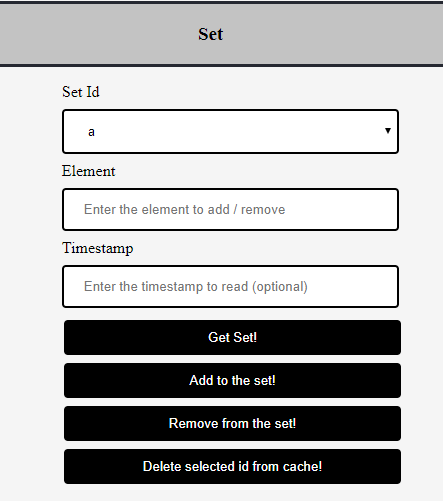
\includegraphics[width=0.6\linewidth]{images/screens/Overview.PNG}}}%
    {\scriptsize}
    \caption {A Set CRDT part of the demonstration application, based on WebCure.}
    \label{fig:dev2}
\end{center}
\end{figure}
 

For each of the supported CRDTs, there are different commands available. In \figref*{fig:dev2}, we can observe the commands that are available for a Set CRDT in our demonstration application. For the explanation of the functionality, there are three inputs available to the user. The first input labelled \textit{Set Id}, is responsible for the names of the elements stored in the local cache and the AntidoteDB. The second input, \textit{Element}, is there for the user to enter a list of elements to add or remove from the Set CRDT. The last input gives an opportunity to provide a specific timestamp, in order to be able to get the data at that timestamp or, in the other case, to apply a selected operation at that timestamp. Apart from the inputs, there are four buttons, which perform specific operations on a set CRDTs -- \textit{getting the value by id}, \textit{adding and removing elements}, \textit{removing element by id from the cache}.

However, for all this functionality to work as intended in both modes -- offline and online -- at first, a service worker has to be set up. 

\subsection*{Setting up a service worker}

Our service worker is located in the root directory of the application under the file \textit{sw.js}. With its help, the application can maintain its main features such as support the offline work and synchronising the changes performed offline with the primary database. As explained in \chapref*{Technologies}, we registered the service worker on \textit{load} event of the application. Then, we added two listeners to the service worker for the events \textit{install} and \textit{fetch}, which we are going to explain further.

\begin{lstlisting}[caption={Code for caching necessary data for the client.}, label={lst:dev4}]
self.addEventListener('install', function(event) {
  // Mention URLS that need to be cached
  // It is required in order for the application to work offline
  var urlsToCache = [
    // root
    '/',
    '/index.html',
    // js
    '/logger.js',
    '/main.js',
    '/dbhelper.js',
    '/idb.js',
    // js CRDTs
    '/CRDTs/CounterCRDT.js',
    '/CRDTs/SetCRDT.js',
    '/CRDTs/MVRegisterCRDT.js',
    // css
    '/styles.css',
    // images
    'img/icon-192.png',
    'img/icon-512.png',
    'img/favicon.ico',
    // manifest
    'manifest.json'
  ];

  event.waitUntil(
    caches.open(CACHES_NAME).then(function(cache) {
      // Add all mentioned urls to the cache, so the app could work without the internet
      return cache.addAll(urlsToCache);
    })
  );
});
\end{lstlisting}

In \lstref*{lst:dev4}, we can see that the array \textit{urlsToCache} consists of elements of type JavaScript strings, which are all the required frameworks, libraries, HTML pages, CSS styles and images needed for the application to work. This array is later used at the \textit{line 28} to create a cache storage \textit{CACHES\_NAME}, where the responses to stored URLs from the array \textit{urlsToCache} are going to be stored. All this work is performed when the installation of the service worker for the page is triggered, which in our case is the start of the application. 

\begin{lstlisting}[caption={Code for maintaining the requests of the application.}, label={lst:dev5}]
self.addEventListener('fetch', function(event) {
  event.respondWith(
    caches.match(event.request).then(function(response) {
      // Respond the data from the cache, if it was found there. Otherwise, fetch from the network.
      return response || fetch(event.request);
    })
  );
});
\end{lstlisting}

Now, once we already have the cached data, we still need to make use of it to make our application work offline. If we look at \lstref*{lst:dev5}, we can see that whenever there is a request going to the network, at \textit{line 3} we are trying to match that request with the ones we have in cache: if it is the case, then the cached object is returned or, otherwise, the fetching process from the network continues, as can be seen at the \textit{line 5}. If the requested resource is not cached and, moreover, the client is offline, then the \textit{fetch} request executes normally and will respond with an error, as the resource will not be loaded.

Apart from caching scripts and media files, necessary for the application to work, we will also need to set up a local database to store the data on the client side.

\subsection*{Setting up a local database}

As explained in \chapref*{Technologies}, in the file \textit{js/dbhelper.js} we are setting up an IndexedDB database for the client side. There, we are going to create two object stores. The first one will consist of different CRDT data items, differentiated by their \textit{id}. The other object store will keep track of the timestamp, which is associated with the latest data taken from the server. The point of having that timestamp is for the client to send it with the updates performed while offline, which will give an insight to the server, at what timestamp these updates should be applied.

\begin{lstlisting}[caption={[Creating object stores in IndexedDB]Creating object stores in IndexedDB for CRDTs and timestamps.}, label={lst:dev6}]
// ...
var stateStore = upgradeDB.createObjectStore('crdt-states', \{
  keyPath: 'id'
\});

var snapshotStore = upgradeDB.createObjectStore('crdt-timestamps', \{
  keyPath: 'id'
\});
// ...
\end{lstlisting}

We can observe the logic explained above in \lstref*{lst:dev6}, where there is an object store named \textit{`crdt-states'} created for CRDTs and \textit{`crdt-timestamps'} for the timestamp. A \textit{keyPath} parameter for both of them is there in order to be able to query the data by \textit{id}. 

While it is clear why do we store the states of CRDTs, it might be not the case for why it is done for the timestamps. First of all, any updates a client makes when it loses the internet connection will be stored in the cache. However, when these updates are sent to the server, it needs to know how to apply them. To that point, the server might have already received updates from some other clients. Therefore, to make sure that the updates we send are applied at the version of the data we were dealing with locally, a client has to provide a timestamp to the server. Secondly, we store a timestamp in the cache for the persistence. While we could have turned to create a variable for this case, it would not have allowed us to use this information after closing the application. Caching solves this problem.

\subsection*{Implementation of abstract Set CRDT}

Next, let us introduce our implementation of Set CRDTs abstraction for the client side, which helps to maintain the data received by the server.

\begin{lstlisting}[caption={[Code for the implementation of \textit{SetCRDT} class]A class \textit{SetCRDT}, objects of which are going to be stored in the \textit{`crdt-states'} object store.}, label={lst:dev7}]
class SetCRDT {
  constructor(id, values) {
    this.id = id;
    this.state = values ? new Set(values) : new Set();
    this.type = 'set';
    this.operations = [];
    this.sentOperations = [];
  }

  processSentOperations() {
    this.operations.forEach(operation => {
      this.sentOperations.push(operation);
    });
    this.operations = [];
  }

  materialize() {
    let values = [];

    this.sentOperations.forEach(operation => {
      if (operation.type === 'add') {
        this.state.add(operation.value);
      } else if (operation.type === 'remove') {
        this.state.delete(operation.value);
      }
    });

    this.operations.forEach(operation => {
      if (operation.type === 'add') {
        this.state.add(operation.value);
      } else if (operation.type === 'remove') {
        this.state.delete(operation.value);
      }
    });

    this.state.forEach(key => {
      values.push(key);
    });

    return values;
  }

  add(valueToAdd) {
    let operation = {
      type: 'add',
      value: valueToAdd
    };

    this.operations.push(operation);
  }

  remove(valueToRemove) {
    let operation = {
      type: 'remove',
      value: valueToRemove
    };

    this.operations.push(operation);
  }
}
\end{lstlisting}

First, let us have a look at the constructor of a \textit{SetCRDT} class in \lstref*{lst:dev7}, which takes two parameters -- an \textit{id} and, optionally, an array of elements -- \textit{values}. The class has the following properties: 

         \begin{itemize}
         \item \textit{id} -- a string corresponding to the id of the data element stored in the server's database;
         \item \textit{state} -- a JavaScript Set, which reflects the state of the \textit{SetCRDT} object and behaves like sets;
	\item \textit{type} -- a string reflecting the datatype and is needed for the client to distinguish between different CRDTs;
	\item \textit{operations} -- an array, which consists of operations performed offline at the client;
	\item \textit{sentOperations} -- an array, which consists of operations performed offline, but which are already sent to the server;
     \end{itemize}

Secondly, there are the methods, which ease the process of working with \textit{Set CDRT} objects at the client: 

         \begin{itemize}
         \item \textit{processSentOperations()} -- shifts offline performed operations to the \textit{sentOperations} property in order to have a distinction for the operations, which are already sent to the client.
         \item \textit{materialize()} -- returns the current state of the CRDT Set, taking into account the operations performed offline.
         \item \textit{add(valueToAdd)} -- performs an offline operation of adding an element to the Set CRDT, takes \textit{valueToAdd} as a parameter.
          \item \textit{remove(valueToRemove)} -- performs an offline operation of removing an element from the Set CRDT, takes \textit{valueToRemove} as a parameter.
     \end{itemize}

\begin{lstlisting}[caption={An example of a \textit{SetCRDT} object, stored on a client side.}, label={lst:dev8}]
{
id: "a",
operations: [{type: "add", value: "c"}],
sentOperations: [],
state: Set(2) {"b", "d"},
type: "set"
}
\end{lstlisting}
     
Having now understood the structure of the data stored on a client side, as well as the way it is managed, let us look at \lstref*{lst:dev8}, where an example of a Set CRDT element with an id \textit{a} is shown. As can be seen, it has a state received from the server of \textit{\{``b'', ``d''\}}, while also having an offline operation \textit{add(c)} performed on it, which is still about to be sent to the server, as an array \textit{sentOperations} is empty at this example.

As we have already explained the server's side logic earlier, in the following sections, we will only touch the topic of a client's offline work and the logic happening at the client on a transition from offline to online modes. We believe that the part, which is related to the online work of the client is already apparent to the reader, as it comes down to the simple client-server communication through predefined requests and this part was already covered when explaining the server's side. 

\subsection*{Read}

One of the crucial aspects of the client working offline as intended is storing the CRDT states received from the server. Let us further explain the logic behind the implementation of it.

\begin{lstlisting}[caption={[Caching on a client side CRDT states, received from the server]Storing CRDT states in the local database after a successful request from the server.}, label={lst:dev9}]
DBHelper.crdtDBPromise
  .then(function(db) {
  // ...

    var tx = db.transaction('crdt-states', 'readwrite');
    var store = tx.objectStore('crdt-states');

    var item = new SetCRDT(id, value);

    store.put(item);

// ...

    return tx.complete;
  })
  .then(function() {
    DBHelper.crdtDBPromise.then(function(db) {
// ...

     var tx = db.transaction('crdt-timestamps', 'readwrite');
     var store = tx.objectStore('crdt-timestamps');
     
     store.put({ id: 0, data: lastCommitTimestamp });

     return tx.complete;
    });
  });
\end{lstlisting}

In \lstref*{lst:dev9}, \textit{DBHelper.crdtDBPromise} at the \textit{line 1} gives us an access to the IndexedDB database consisting the object stores we created. There, we start a transaction on a \textit{`crdt-states'} object store and at the \textit{line 8} we create an element of \textit{SetCRDT} class introduced above, passing it the \textit{id} of the Set CRDT and its \textit{value} that was just received from the server. Then we assign it to the variable \textit{item} and add this \textit{item} to the object store of CRDT states using the method \textit{put} of \textit{store} object. Next, we close the transaction using the method \textit{complete} of the \textit{tx} transaction object.

When we successfully stored the received state, there is another piece of information that has to be saved on the client as well. This time it is a timestamp associated with the update we received. Looking again at \lstref*{lst:dev9}, at \textit{line 20} we refer to the \textit{`crdt-timestamps'} object store this time. Similarly as before, as can be seen at the \textit{line 25}, we store \textit{lastCommitTimestamp}, which consists the timestamp received from the server. That happens each time we get a new update from the server and normally, there is no way to observe a new update without an updated timestamp as well.


\begin{lstlisting}[caption={Reading CRDT states from client's cache.}, label={lst:dev10}]
DBHelper.crdtDBPromise.then(function(db) {
// ...

  var index = db.transaction('crdt-states').objectStore('crdt-states');

  return index.get(id).then(function(state) {
    if (state) {
     Object.setPrototypeOf(state, SetCRDT.prototype);
     log('[Offline] The value of ' + name.value + 'is: [ ' + state.materialize() + ']');
    } else {
     log('[Offline] Selected key is not available offline.');
    }
  });
});
\end{lstlisting}

Now comes the part regarding reading the states of the Set CRDTs from the cache. We can have a look at \lstref*{lst:dev10}, where the code already looks familiar to us. There, at the \textit{line 6}, we use the method \textit{get} of \textit{index} to search by the property \textit{id} of the object. Then, if an element with such \textit{id} was found in the object store, we are going to have it in a \textit{state} variable. As we do not store the class information in the client's database, we will have to ``remind'' the object we have in the \textit{state} variable about its prototype. That is why a method \textit{Object.setPrototypeOf} is used with \textit{state} and \textit{SetCRDT.prototype} as parameters. After that, the object \textit{state} will have an access to the methods of a \textit{SetCRDT} class. For the demonstration of the client's functionality, in this thesis we are using a JavaScript Logger\footnote{http://www.songho.ca/misc/logger/logger.html} library, which we have an access to under the \textit{log} variable at \textit{lines 9 and 11}. It let us keep the track of neccessary information in a convinient manner. As can be seen, at the \textit{line 9} we log the actual state of the Set CRDT using a \textit{materialize()} method of \textit{SetCRDT} class.

\subsection*{Add / Remove}

Another functionality that a client covers, apart from reading and storing the values in the local database, it is performing the operations on CRDTs offline.

\begin{lstlisting}[caption={[Applying operation \textit{add} on a Set CRDT while offline]Performing an operation \textit{add} on a Set CRDT while the client is offline.}, label={lst:dev11}]
DBHelper.crdtDBPromise
  .then(function(db) {
// ...

    var index = db.transaction('crdt-states').objectStore('crdt-states');

    return index.get(id).then(function(storedValue) {
      var tx = db.transaction('crdt-states', 'readwrite');
      var store = tx.objectStore('crdt-states');

      Object.setPrototypeOf(storedValue, SetCRDT.prototype);
      storedValue.add(value);
      store.put(storedValue);

      return tx.complete;
    });
  });
\end{lstlisting}

Looking at \lstref*{lst:dev11}, we can see that there is not so much of a difference with previous code that we have seen on performing the read operations from IndexedDB. Again, as we can see from the example, a transaction on a \textit{`crdt-states'} object store is created and if an element with \textit{id} is found in the object store, its value will be available under the variable \textit{storedValue}. Then, similarly, the method \textit{Object.setPrototypeOf} is used for the \textit{storedValue}, in order for it to have an access to the \textit{SetCRDT} class methods. Once it is done, at \textit{line 12} we use the method \textit{storedValue.add(value)}, where \textit{value} variable is the value entered by the user. If we get back to \lstref*{lst:dev7}, we will recall that the method \textit{add} will add an element to the array-type property \textit{operations} of the object \textit{storedValue}. Finally, we use \textit{store.put(storedValue)} to put the update data item back to the client's database and afterwards complete the transaction. Similarly, the same happens when a user tries to remove elements from Set CRDTs.

\subsection*{A transition from offline to online}

Next, we would like to discuss what happens when the client switches from offline mode back to online. For every offline operation performed on sets, we register a unique tag named \textit{syncSetChanges}, as was explained in \secref*{BackgroundSync}.

\begin{lstlisting}[caption={[A function, which synchronises operations with the server when the connection is re-established]A function \textit{pushSetChangesToServer}, triggered whenever a client reconnects to the network.}, label={lst:dev12}]
function pushSetChangesToServer() {
  // ...
  DBHelper.crdtDBPromise.then(function(db) {
    var index = db.transaction('crdt-states').objectStore('crdt-states');

    return index
      .getAll()
      .then(function(objects) {
        DBHelper.crdtDBPromise.then(function(db) {
          // ...
          var index = db.transaction('crdt-timestamps').objectStore('crdt-timestamps');
          return index.get(0).then(function(timestamp) {
            if (objects) {
              objects.forEach(object => {
                if (object.operations.length > 0) {
                  fetch(`${DBHelper.SERVER_URL}/api/set_sync/${object.id}`, {
                    method: 'POST',
                    body: JSON.stringify({
                      lastCommitTimestamp: timestamp ? timestamp : undefined,
                      updates: object.operations
                    }),
                    headers: {
                      'Content-Type': 'application/json; charset=utf-8'
                    }
                  });
                }
              });
            }
          });
        });
      })
      .then(function() {
        return DBHelper.crdtDBPromise.then(function(db) {
          // ...

       var index = db.transaction('crdt-states').objectStore('crdt-states');

       return index.getAll().then(function(objects) {
         var tx = db.transaction('crdt-states', 'readwrite');
         var store = tx.objectStore('crdt-states');
         if (objects) {
              objects.forEach(object => {
                if (object.type === 'set') {
                  Object.setPrototypeOf(object, SetCRDT.prototype);
                  object.processSentOperations();
                  store.put(object);
                }
              });
            }
         return tx.complete;
          });
        });
      });
  });
}
\end{lstlisting}

Then, a \textit{sync} event is going to be triggered inside the service worker. At the time it happens, we are going to check whether our tag \textit{syncSetChanges} registered it. In this case, a function \textit{pushSetChangesToServer} is called, which we can observe at \lstref*{lst:dev12}. 

Let us have a closer look into it. At the \textit{line 7}, we get all the elements stored in the object store of \textit{`crdt-states'}. In this section, we are describing the implementation of maintaining only Set CRDTs. However, the object store \textit{`crdt-states'} normally can contain any CRDTs. Once we got the states, at \textit{line 12}, we are also getting the latest timestamp that was stored on a client side (we use \textit{get(0)} here, as we store every new timestamp under the id \textit{0}). This step is specifically needed for the causality of updates (more details are available in \chapref*{Design}). Then, for every Set CRDT, we are creating a POST HTTP request, which contains the information about the timestamp at which these updates were performed, as well as operations themselves. We can see it at \textit{lines 16--24}, where the timestamp is sent as \textit{lastCommitTimestamp} and operations are sent as \textit{object.operations}. In such a way, this information is sent to the server, which continues processing it on its side.

However, this is not it for the client yet. There is a reason why the client has to distinguish between offline operations that are already sent to the server and the ones that are not yet. First of all, in order to not send the same updates multiple times to the server. At the \textit{line 46} of \lstref*{lst:dev12}, we see that the method \textit{processSentOperations()} is called. We can look up its implementation again in \lstref*{lst:dev7}. As we remember, it shifts already sent operations to another array named \textit{sentOperations}, which is also a property of the class \textit{SetCRDT}. Our reader might also think about the possibility of just clearing these operations from the cache as soon as the internet connection at the client side is re-established again. That would not be a good idea. Let us imagine the following situation: a client works offline for some time, then the connection gets back, but before the client could request new updates from the server, the connection gets off again. What happens in such a scenario? First of all, the operations performed offline at the client side will be sent to the server immediately, but if we delete from the cache operations that are sent already, then we are risking losing the data at client side. As we did not yet receive the latest updates from the server, the client would not be able to continue working offline on its data. It was the second reason, why it is better to keep offline operations at client side in two separate collections, at least before the server sends back data updates, having already applied the operations, which the client sent. At that point, it will be safe to remove them.

Finally, we have covered so far every aspect of the implementation, and in the next chapter, we will evaluate our work.